\documentclass[11pt, a4paper, norsk]{NTNUoving}
\usepackage[utf8]{inputenc}
\usepackage[T1]{fontenc}
\usepackage{placeins}

\ovingnr{4}    % Nummer på innlevering
\semester{Høsten 2019}
\fag{TMA 4110}
\institutt{Institutt for matematiske fag}

\begin{document}
   \begin{oppgave}
       Hvilke matriser representerer projeksjoner?
       
      For å finne ut om en matrise representerer en projeksjon, må jeg sjekke om matrisen ganget med seg selv er den samme matrisen. Jeg gjør dette i alle deloppgavene i denne oppgaven.
       \begin{punkt}
           $
           \begin{bmatrix}
               0 & 0 \\
               1 & 1
           \end{bmatrix}
           $

           \begin{align*}
                \begin{bmatrix}
                    0 & 0 \\
                    1 & 1
                \end{bmatrix}^2 = \begin{bmatrix}
                    0 & 0 \\
                    1 & 1
                \end{bmatrix}            
           \end{align*}
           Ja, denne matrisen representerer en projeksjon.
       \end{punkt}
       \begin{punkt}
           $
            \begin{bmatrix}
                0 & 0 \\
                2 & 1
            \end{bmatrix}
           $
           \begin{align*}
                \begin{bmatrix}
                    0 & 0 \\
                    2 & 1
                \end{bmatrix}^2 = \begin{bmatrix}
                    0 & 0 \\
                    2 & 1
                \end{bmatrix}
           \end{align*}
           Ja, denne matrisen representerer en projeksjon
       \end{punkt}
       \begin{punkt}
           $
            \begin{bmatrix}
                0 & 0 \\
                0 & 1
            \end{bmatrix}
           $
           \begin{align*}
                \begin{bmatrix}
                    0 & 0 \\
                    0 & 1
                \end{bmatrix}^2 = \begin{bmatrix}
                    0 & 0 \\
                    0 & 1
                \end{bmatrix}
           \end{align*}
           Ja, denne matrisen representerer en projeksjon
       \end{punkt}
       \begin{punkt}
            $
                \begin{bmatrix}
                    0 & 0 \\
                    1 & 0
                \end{bmatrix}
            $
            \begin{align*}
                \begin{bmatrix}
                    0 & 0 \\
                    1 & 0
                \end{bmatrix}^2 = \begin{bmatrix}
                    0 & 0 \\
                    0 & 0
                \end{bmatrix}
            \end{align*}
            Nei, denne matrisen representerer ikke en projeksjon.
       \end{punkt}
       \begin{punkt}
           $
           \begin{bmatrix}
               0 & 1 \\
               1 & 0
           \end{bmatrix}
           $
       \end{punkt}
       \begin{align*}
           \begin{bmatrix}
               0 & 1 \\
               1 & 0
           \end{bmatrix}^2 = \begin{bmatrix}
               1 & 0 \\
               0 & 1
           \end{bmatrix}
       \end{align*}
       Nei, denne matrisen representerer ikke en projeksjon.
       \begin{punkt}
           $
            \begin{bmatrix}
               1 & 0 \\
               0 & 1
           \end{bmatrix}
           $
       \end{punkt}
       \begin{align*}
           \begin{bmatrix}
               1 & 0 \\
               0 & 1
           \end{bmatrix}^2 = \begin{bmatrix}
               1 & 0 \\
               0 & 1
           \end{bmatrix}
       \end{align*}
       Ja, denne matrisen representerer en projeksjon.
   \end{oppgave}
   \begin{oppgave}
       Hvilke av vektorene er ortogonale med hverandre?
       
       I disse deloppgavene må jeg ta prikkproduktet mellom vektorene og sjekke om de er lik 0.
       \begin{punkt}
           $
            \begin{bmatrix}
                2 \\
                -5 \\
                1
            \end{bmatrix}
           $ og $
            \begin{bmatrix}
                1 \\
                2 \\
                0
            \end{bmatrix}
           $
           Prikkproduktet:
           \begin{align*}
               \begin{bmatrix}
                   2 \\
                   -5 \\
                   1
               \end{bmatrix} \cdot \begin{bmatrix}
                   1 \\
                   2 \\
                   0
               \end{bmatrix} &= 2 \cdot 1 + (-5) \cdot 2 + 0
               \\
               &= -8
           \end{align*}
           Nei, disse vektorene er ikke ortogonale.
       \end{punkt}
       \begin{punkt}
           $\begin{bmatrix}
               1 \\
               0 \\
               -1
           \end{bmatrix}$, $\begin{bmatrix}
               1 \\
               \sqrt{2} \\
               1
           \end{bmatrix}$ og $\begin{bmatrix}
               1 \\
               -\sqrt{2} \\
               1
           \end{bmatrix}$
           Her må jeg sjekke to og to:
           \begin{align*}
               \begin{bmatrix}
                   1 \\
                   0 \\
                   -1
               \end{bmatrix} \cdot \begin{bmatrix}
                   1 \\
                   \sqrt{2} \\
                   1
               \end{bmatrix} &= 1 \cdot 1 + 0 + -1 \cdot 1
               \\
               &= 0
               \\
               \\
               \begin{bmatrix}
                   1 \\
                   0 \\
                   -1
               \end{bmatrix} \cdot \begin{bmatrix}
                   1 \\
                   -\sqrt{2} \\
                   1
               \end{bmatrix} &= 1 \cdot 1 + 0 + -1 \cdot 1
               \\
               &= 0
               \\
               \\
               \begin{bmatrix}
                   1 \\
                   \sqrt{2} \\
                   1
               \end{bmatrix} \cdot \begin{bmatrix}
                   1 \\
                   -\sqrt{2} \\
                   1
               \end{bmatrix} &= 1 \cdot 1 + \sqrt{2} \cdot -\sqrt{2} + 1 \cdot 1 \\
               &= 0
           \end{align*}
           Ja, disse vektorene er ortogonale.
       \end{punkt}
       \begin{punkt}
           $\begin{bmatrix}
               i \\
               0 \\
               1
           \end{bmatrix}$, $\begin{bmatrix}
               i \\
               1 \\
               0
           \end{bmatrix}$ og $\begin{bmatrix}
               1 \\
               i \\
               i
           \end{bmatrix}$

           Her må jeg også sjekke to og to. Samtidig, når en skal ta prikkproduktet til komplekse vektorer, må en adjungere den ene:
           \begin{align*}
               \begin{bmatrix}
                   i \\
                   0 \\
                   1
               \end{bmatrix} \cdot \begin{bmatrix}
                   i \\
                   1 \\
                   0
               \end{bmatrix} &= \begin{bmatrix}
               -i & 0 & 1
               \end{bmatrix} \cdot \begin{bmatrix}
                   i \\
                   1 \\
                   0
               \end{bmatrix}
               \\
               &= -i \cdot i + 0 \cdot 1 + 1\cdot 0
               \\
               &= 1 \neq 0
           \end{align*}
           Nei, disse vektorene er ikke ortogonale.
       \end{punkt}
   \end{oppgave}
   \begin{oppgave}
       Bruk Gram-Schmidts metode for å finne en ortogonal basis med utgangspunkt i:
       \begin{punkt}
           Vektorene oppgitt i oppgave 2a:

           Starter med å sette $\underline{u_1} = \begin{bmatrix}
               2 \\
               -5 \\
               1
           \end{bmatrix}$. Finner $\underline{u_2}$:
           \begin{align*}
               \underline{u_2} &= \underline{v_2} - \frac{<\underline{u_2}, \underline{v_2}>}{<\underline{u_1}, \underline{u_1}>}
               \\
                               &= \begin{bmatrix}
                                   1 \\
                                   2 \\
                                   0
                               \end{bmatrix} - -\frac{8}{30}\cdot \begin{bmatrix}
                                   2 \\
                                   -5 \\
                                   1
                               \end{bmatrix}
                               \\
                               &= \begin{bmatrix}
                                   1 \\
                                   2 \\
                                   0
                               \end{bmatrix} - \begin{bmatrix}
                                   -\frac{8}{15} \\
                                   \frac{4}{3} \\
                                   -\frac{4}{15}
                               \end{bmatrix}
                               \\
                               &= \begin{bmatrix}
                                   \frac{23}{15} \\
                                   \frac{2}{3} \\
                                   \frac{4}{15}
                               \end{bmatrix}
                               \\
                               \text{Sjekker at de er ortogonale:}
                               \\
                               \\
                               \begin{bmatrix}
                                   2 \\
                                   -5 \\
                                   1
                               \end{bmatrix} \cdot \begin{bmatrix}
                                   \frac{23}{15} \\
                                   \frac{2}{3} \\
                                   \frac{4}{15}
                               \end{bmatrix} &= 2 \cdot \frac{23}{15} + -5 \cdot \frac{2}{3} + 1 \cdot \frac{4}{15}
                               \\
                               &= 0
           \end{align*}
           En ortogonal basis for vektorene i oppgave 2a er $Sp\left\{\begin{bmatrix}
               2 \\
               -5 \\
               1
           \end{bmatrix}, \begin{bmatrix}
               \frac{23}{15} \\
               \frac{2}{3} \\
               \frac{4}{15}
           \end{bmatrix}\right\}$
       \end{punkt}
       \begin{punkt}
           Vektorene oppgitt i oppgave 2b.

           Disse vektorene er allere ortogonale. De er allere en ortogonal basis.
       \end{punkt}
       \begin{punkt}
            Vektorene oppgitt i oppgave 2c.

            Starter med $\underline{u_1} = \begin{bmatrix}
                i \\
                0 \\
                1
            \end{bmatrix}$. Finner $\underline{u_2}$:
            \begin{align*}
                \underline{u_2} &= \begin{bmatrix}
                    i \\
                    1 \\ 
                    0
                \end{bmatrix} - \frac{\begin{bmatrix}
                    -i & 0 & 1
                \end{bmatrix} \cdot \begin{bmatrix}
                    i \\
                    1 \\
                    0
                \end{bmatrix}}{\begin{bmatrix}
                    -i & 0 & 1
                \end{bmatrix} \cdot \begin{bmatrix}
                    i \\
                    0 \\
                    1
                \end{bmatrix}} \cdot \begin{bmatrix}
                    i \\
                    0 \\
                    1
                \end{bmatrix} 
                \\
                                &= \begin{bmatrix}
                                    i \\
                                    1 \\
                                    0
                                \end{bmatrix} - \frac{1}{2} \cdot \begin{bmatrix}
                                    i \\
                                    0 \\
                                    1
                                \end{bmatrix}
                                \\
                                &= \begin{bmatrix}
                                    i \\
                                    1 \\
                                    0
                                \end{bmatrix} - \begin{bmatrix}
                                    \frac{i}{2} \\
                                    0 \\
                                    \frac{1}{2}
                                \end{bmatrix}
                                \\
                                &= \begin{bmatrix}
                                    \frac{i}{2} \\
                                    0 \\
                                    \frac{-1}{2}
                                \end{bmatrix}
                                \\
                                \\
                    \underline{u_3} &= \begin{bmatrix}
                        1 \\
                        i \\
                        i
                    \end{bmatrix} - \frac{\begin{bmatrix}
                        -i & 0 & 1
                    \end{bmatrix} \cdot \begin{bmatrix}
                        1 \\
                        i \\
                        i
                    \end{bmatrix}}{2} \cdot \begin{bmatrix}
                        i \\
                        0 \\
                        1
                    \end{bmatrix} - \frac{\begin{bmatrix}
                        \frac{-i}{2} & 1 & \frac{-1}{2}
                    \end{bmatrix} \cdot \begin{bmatrix}
                        1 \\
                        i \\
                        i
                    \end{bmatrix}}{\begin{bmatrix}
                        \frac{-i}{2} & 1 & \frac{-1}{2}
                    \end{bmatrix} \cdot \begin{bmatrix}
                        \frac{i}{2} \\
                        1 \\
                        \frac{-1}{2}
                    \end{bmatrix}} \cdot \begin{bmatrix}
                        \frac{i}{2} \\
                        1 \\
                        \frac{-1}{2}
                    \end{bmatrix}
                    \\
                                    &= \begin{bmatrix}
                                        1 \\
                                        i \\
                                        i
                                    \end{bmatrix} - \underline{0} - \underline{0}
                                    \\
                                    &= \begin{bmatrix}
                                        1 \\
                                        i \\
                                        i
                                    \end{bmatrix}
            \end{align*}
            En ortogonal basis for vektorene i oppgave 2c er $Sp\left\{\begin{bmatrix}
                i \\
                0 \\
                1
            \end{bmatrix}, \begin{bmatrix}
                \frac{i}{2} \\
                1 \\
                \frac{-1}{2}
            \end{bmatrix}, \begin{bmatrix}
                1 \\
                i \\
                i
            \end{bmatrix}\right\}$
       \end{punkt}
   \end{oppgave}
   \begin{oppgave}
       Hva blir den ortogonale projeksjonen av
       \begin{punkt}
           $\begin{bmatrix}
               1 \\
               2 \\
               3
           \end{bmatrix}$ ned på vektorene gitt i 2a?

           Jeg finner den ortogonale projeksjonen ved:

           $P_{u}\left(\begin{bmatrix}
               1 \\
               2 \\
               3
       \end{bmatrix}\right) = P_{v_1}\left(\begin{bmatrix}
           1 \\
           2 \\
           3
       \end{bmatrix}\right) + P_{v_2}\left(\begin{bmatrix}
           1 \\
           2 \\
           3
   \end{bmatrix}\right)$. Jeg har basisen jeg fant i forrige oppgave (den ene vektoren skalert med $15$ for å bli kvitt brøk.):
           \begin{align*}
               P_{u} &= \frac{\begin{bmatrix}
                   23 \\
                   10 \\
                   4
               \end{bmatrix} \cdot \begin{bmatrix}
                   1 \\
                   2 \\ 
                   3
               \end{bmatrix}}{\begin{bmatrix}
                   23 \\
                   10 \\
                   4
               \end{bmatrix} \cdot \begin{bmatrix}
                   23 \\
                   10 \\
                   4
               \end{bmatrix}} \cdot \begin{bmatrix}
                   23 \\
                   10 \\
                   4
               \end{bmatrix} + \frac{\begin{bmatrix}
                   2 \\
                   -5 \\
                   1
               \end{bmatrix} \cdot \begin{bmatrix}
                   1 \\
                   2 \\
                   3
               \end{bmatrix}}{\begin{bmatrix}
                   2 \\
                   -5 \\
                   4
               \end{bmatrix} \cdot \begin{bmatrix}
                   2 \\
                   -5 \\
                   5
               \end{bmatrix}} \cdot \begin{bmatrix}
                   2 \\
                   -5 \\
                   1
               \end{bmatrix}
               \\
                     &= \frac{23 + 20 + 12}{23^2 + 10^2 + 4^2} \cdot \begin{bmatrix}
                         23 \\
                         10 \\
                         4
                     \end{bmatrix} + \frac{2 - 10 + 3}{2^2 + (-5)^2 + 1^2} \cdot \begin{bmatrix}
                         2 \\
                         -5 \\
                         1
                     \end{bmatrix}
                     \\
                     &= \frac{11}{129} \cdot \begin{bmatrix}
                         23 \\
                         10 \\
                         4
                     \end{bmatrix} - \frac{1}{6} \cdot \begin{bmatrix}
                         2 \\
                         -5 \\
                         1
                     \end{bmatrix}
                     \\
                     &= \begin{bmatrix}
                         \frac{70}{43} \\
                         \frac{145}{86} \\
                         \frac{15}{86}
                     \end{bmatrix} = \begin{bmatrix}
                         140 \\
                         145 \\
                         15
                     \end{bmatrix} = \begin{bmatrix}
                         28 \\
                         29 \\
                         3
                     \end{bmatrix}
           \end{align*}
           Den ortogonale projeksjonen av $\begin{bmatrix}
               1 \\
               2 \\
               3
           \end{bmatrix}$ ned på vektorene i 2a er $\begin{bmatrix}
               28 \\
               29 \\
               3
           \end{bmatrix}$
       \end{punkt}
       \begin{punkt}
           $\begin{bmatrix}
               2 \\
               \sqrt{2} \\
               2
           \end{bmatrix}$ ned på vektorene gitt i 2b?

            Har basisen $Sp\left\{\begin{bmatrix}
                1 \\
                0 \\
                -1
            \end{bmatrix}, \begin{bmatrix}
                1 \\
                \sqrt{2} \\
                1
            \end{bmatrix}, \begin{bmatrix}
                1 \\
                -\sqrt{2} \\
                1
        \end{bmatrix}\right\}$ fra oppgave 2b. Jeg finner projeksjonen $P_{u}\left(\begin{bmatrix}
            2 \\
            \sqrt{2} \\
            2
        \end{bmatrix}\right)$:
       
        \begin{align*}
            P_{u}\left(\begin{bmatrix}
                2 \\
                \sqrt{2} \\
                2
            \end{bmatrix}\right) &= \frac{\begin{bmatrix}
                1 \\
                0 \\
                -1
            \end{bmatrix} \cdot \begin{bmatrix}
                2 \\
                \sqrt{2} \\
                2
            \end{bmatrix}}{\begin{bmatrix}
                1 \\
                0 \\
                -1
            \end{bmatrix} \cdot \begin{bmatrix}
                1 \\
                0 \\
                -1
            \end{bmatrix}} \cdot \begin{bmatrix}
                1 \\
                0 \\
                -1
            \end{bmatrix} + \frac{\begin{bmatrix}
                1 \\
                \sqrt{2} \\
                1
            \end{bmatrix} \cdot \begin{bmatrix}
                2 \\
                \sqrt{2} \\
                2
            \end{bmatrix}}{\begin{bmatrix}
                1 \\
                \sqrt{2} \\
                1
            \end{bmatrix} \cdot \begin{bmatrix}
                1 \\
                \sqrt{2} \\
                1
            \end{bmatrix}} \cdot \begin{bmatrix}
                1 \\
                \sqrt{2} \\
                1
            \end{bmatrix} + \frac{\begin{bmatrix}
                1 \\
                -\sqrt{2} \\
                1
            \end{bmatrix} \cdot \begin{bmatrix}
                2 \\
                \sqrt{2} \\
                2
            \end{bmatrix}}{\begin{bmatrix}
                1 \\
                -\sqrt{2} \\
                1
            \end{bmatrix} \cdot \begin{bmatrix}
                1 \\
                -\sqrt{2} \\
                1
            \end{bmatrix}} \cdot \begin{bmatrix}
                1 \\
                -\sqrt{2} \\
                1
            \end{bmatrix}
            \\
            &= \frac{0}{2}\cdot \begin{bmatrix}
                1 \\
                0 \\
                -1
            \end{bmatrix} + \frac{2+2+2}{1+2+1} \cdot \begin{bmatrix}
                1 \\
                \sqrt{2} \\
                1
            \end{bmatrix} + \frac{2-2+2}{1+2+1} \cdot \begin{bmatrix}
                1 \\
                -\sqrt{2} \\
                1
            \end{bmatrix}
            \\
            &= \frac{3}{2} \cdot \begin{bmatrix}
                1 \\
                \sqrt{2} \\
                1
            \end{bmatrix} + \frac{1}{2} \cdot \begin{bmatrix}
                1 \\
                -\sqrt{2} \\
                1
            \end{bmatrix}
            \\
            &= \begin{bmatrix}
                \frac{3}{2} \\
                \frac{3 \cdot \sqrt{2}}{2} \\
                \frac{3}{2}
            \end{bmatrix} + \begin{bmatrix}
                \frac{1}{2} \\
                -\frac{\sqrt{2}}{2} \\
                \frac{1}{2}
            \end{bmatrix} = \begin{bmatrix}
                2 \\
                \sqrt{2} \\
                2
            \end{bmatrix}
        \end{align*}
        Den ortogonale projeksjonen av $\begin{bmatrix}
            2 \\
            \sqrt{2} \\
            2
        \end{bmatrix}$ ned på vektorene i 2b er $\begin{bmatrix}
            2 \\
            \sqrt{2} \\
            2
        \end{bmatrix}$
       \end{punkt}
       \begin{punkt}
           $\begin{bmatrix}
               i \\
               i \\
               i
           \end{bmatrix}$ ned på vektorene i 2c?
           
           Har basisen $Sp\left\{\begin{bmatrix}
               i \\
               0 \\
               1
           \end{bmatrix}, \begin{bmatrix}
               i \\
               2 \\
               -1
           \end{bmatrix}, \begin{bmatrix}
               1 \\
               i \\
               i
           \end{bmatrix}\right\}$. Finner $P_{u}\left(\begin{bmatrix}
               i \\ 
               i \\
               i
       \end{bmatrix}\right)$:
       \begin{align*}
          P_{u}\left(\begin{bmatrix}
               i \\ 
               i \\
               i
       \end{bmatrix}\right) &= \frac{\begin{bmatrix}
       -i & 0 & 1
       \end{bmatrix} \cdot \begin{bmatrix}
           i \\
           i \\
           i
       \end{bmatrix}}{\begin{bmatrix}
       -i & 0 & 1
       \end{bmatrix} \cdot \begin{bmatrix}
           i \\
           0 \\
           1
       \end{bmatrix}} \cdot \begin{bmatrix}
           i \\
           0 \\ 
           1
       \end{bmatrix} + \frac{\begin{bmatrix}
       -i & 2 & -1
       \end{bmatrix} \cdot \begin{bmatrix}
           i \\
           i \\
           i
       \end{bmatrix}}{\begin{bmatrix}
       -i & 2 & -1
       \end{bmatrix} \cdot \begin{bmatrix}
           i \\
           2 \\
           -1
       \end{bmatrix}} \cdot \begin{bmatrix}
           i \\
           2 \\
           -1
       \end{bmatrix} 
       \\
       &+ \frac{\begin{bmatrix}
       1 & -i & -i
       \end{bmatrix} \cdot \begin{bmatrix}
           i \\ 
           i \\
           i
       \end{bmatrix}}{\begin{bmatrix}
       1 & -i & -i
       \end{bmatrix} \cdot \begin{bmatrix}
           1 \\
           i \\
           i
       \end{bmatrix}} \cdot \begin{bmatrix}
           1 \\
           i \\
           i
       \end{bmatrix}
       \\
       &= \frac{1+i}{2} \cdot \begin{bmatrix}
           i \\
           0 \\
           1
       \end{bmatrix} + \frac{1+2i-i}{6} \cdot \begin{bmatrix}
           i \\
           2 \\
           -1
       \end{bmatrix} + \frac{i + 1 + 1}{3} \cdot \begin{bmatrix}
           1 \\
           i \\
           i
       \end{bmatrix}
       \\
       &= \begin{bmatrix}
           i \\
           i \\
           i
       \end{bmatrix}
       \end{align*}
       Den ortogonale projeksjonen av $\begin{bmatrix}
           i \\
           i \\
           i
       \end{bmatrix}$ ned på vektorene i 2c er $\begin{bmatrix}
           i \\
           i \\
           i
       \end{bmatrix}$
       \end{punkt}
   \end{oppgave}
    
   \begin{oppgave}
       La $\underline{u} = \begin{bmatrix}
           2 \\
           -5
       \end{bmatrix}$ og $\underline{v} = \begin{bmatrix}
           1 \\
           2
       \end{bmatrix}$. Finn den ortogonale projeksjonen av $\underline{u}$ på $\underline{v}$. Tegn $\underline{u}$, $\underline{v}$ og projeksjonen i samme koordinatsystem. Hva er vinkelen mellom vektorene?

       Finner $P_{v}(u)$:
       \begin{align*}
           P_{v}(u) &= \frac{2 \cdot 1 + 2 \cdot -5}{1^2 + 2^2} \cdot \begin{bmatrix}
               1 \\
               2
           \end{bmatrix} \\
                    &= \begin{bmatrix}
                        -\frac{8}{5} \\
                        -\frac{16}{5}
                    \end{bmatrix}
       \end{align*}
       \begin{figure}[!ht]
           \centering
           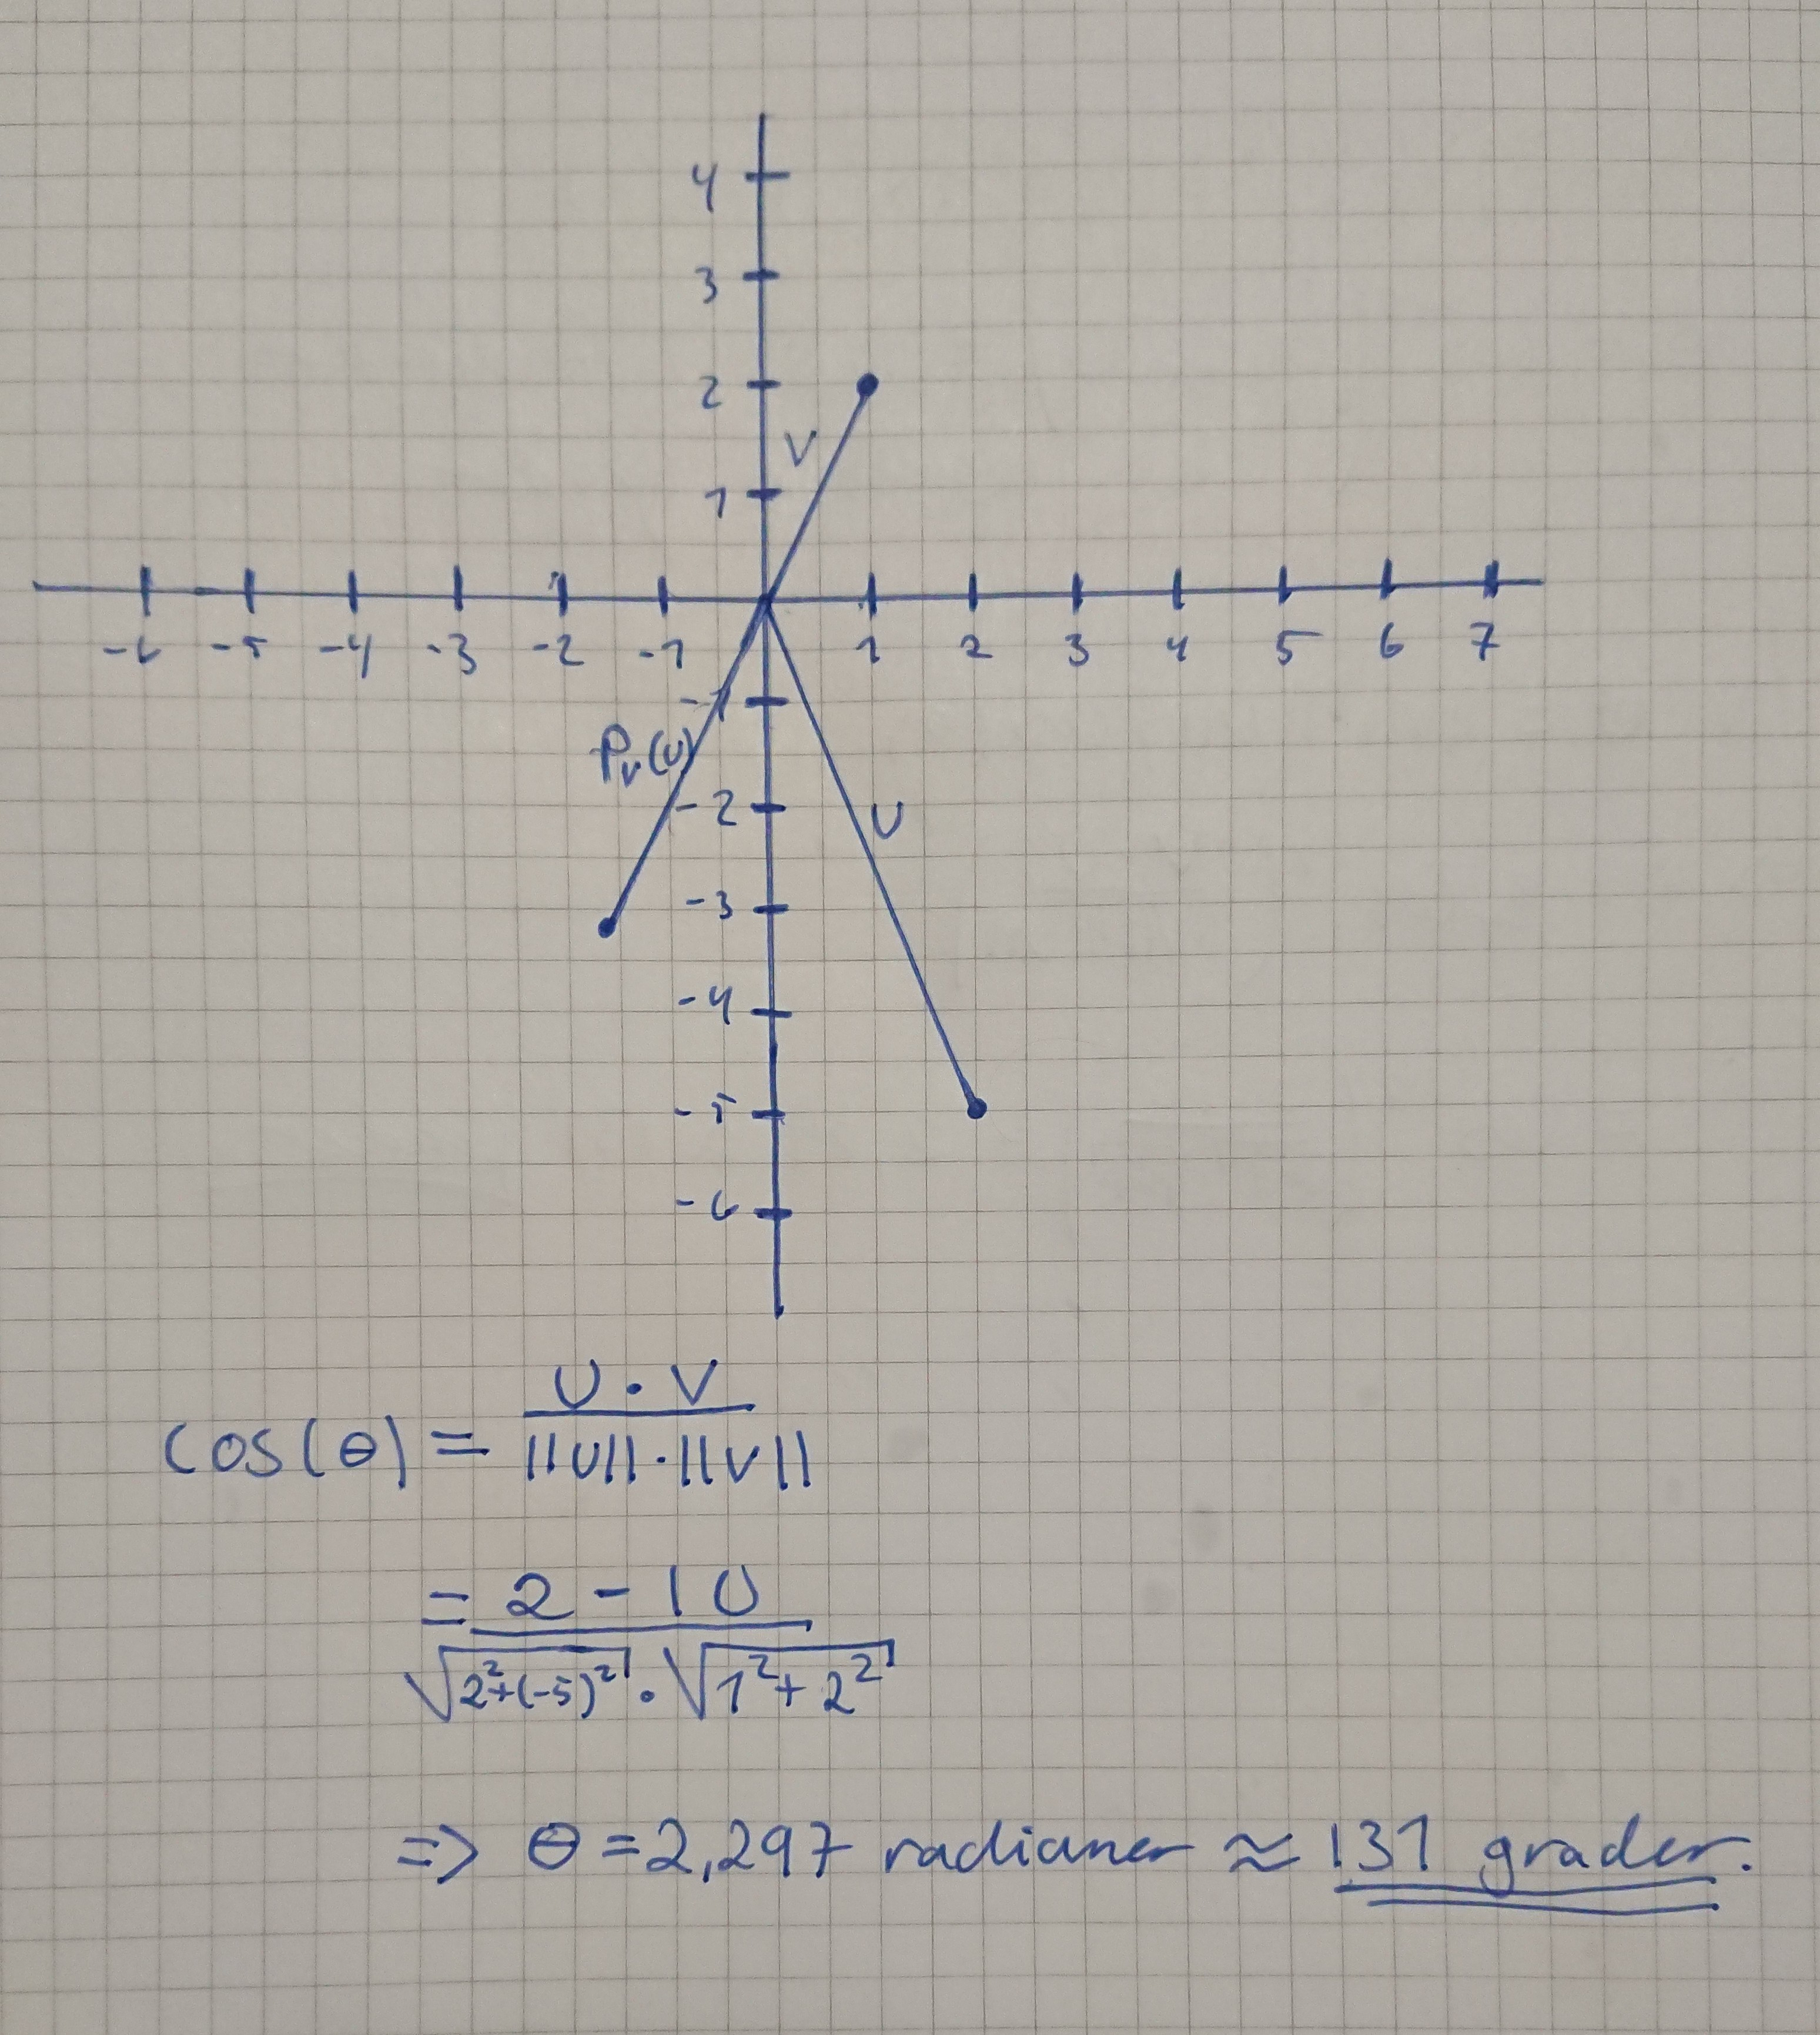
\includegraphics[width=10cm]{oppgave_5.JPG}
           \caption{Oppgave 5}
           \label{fig:oppgave5}
       \end{figure}
       \FloatBarrier
   \end{oppgave}
    \begin{oppgave}
        Beregn $P_{u}(v)$ og $v - P_{u}(v)$ når
        \begin{punkt}
            $\underline{u} = \begin{bmatrix}
                2 \\
                2 \\
                1
            \end{bmatrix}$ og $\underline{v} = \begin{bmatrix}
                3 \\
                2 \\
                1
            \end{bmatrix}$
            \begin{align*}
                P_{\underline{u}}(\underline{v}) &= \frac{2 \cdot 3 + 2 \cdot 2 + 1 \cdot 1}{2^2 + 2^2 + 1^1} \cdot \begin{bmatrix}
                    2 \\
                    2 \\
                    1
                \end{bmatrix}
                \\
                         &= \frac{11}{9} \cdot \begin{bmatrix}
                             2 \\
                             2 \\
                             1
                         \end{bmatrix} = \begin{bmatrix}
                             \frac{22}{9} \\
                             \frac{22}{9} \\
                             \frac{11}{9}
                         \end{bmatrix}
                         \\
                         \\
                    \underline{v} - P_{\underline{u}}(\underline{v}) &= \begin{bmatrix}
                        3 \\
                        2 \\
                        1
                    \end{bmatrix} - \begin{bmatrix}
                        \frac{22}{9} \\
                        \frac{22}{9} \\
                        \frac{11}{9}
                    \end{bmatrix} = \begin{bmatrix}
                        \frac{5}{9} \\
                        -\frac{4}{9} \\
                        -\frac{2}{9}
                    \end{bmatrix}
            \end{align*}
        \end{punkt}
        \begin{punkt}
            $\underline{u} = \begin{bmatrix}
                -1 \\
                2 \\
                -1
            \end{bmatrix}$ og $\underline{v} = \begin{bmatrix}
                1 \\
                3 \\
                1
            \end{bmatrix}$
            \begin{align*}
                P_{\underline{u}}(\underline{v}) &= \frac{-1 + 6 - 1}{6} \cdot \begin{bmatrix}
                    -1 \\
                    2 \\
                    -1
                \end{bmatrix}
                \\
                         &= \frac{4}{6} \cdot \begin{bmatrix}
                             -1 \\
                             2 \\
                             -1
                         \end{bmatrix} = \begin{bmatrix}
                             -\frac{2}{3} \\
                             \frac{4}{3} \\
                             -\frac{2}{3}
                         \end{bmatrix}
                         \\
                         \\
                    \underline{v} - P_{\underline{u}}(\underline{v}) &= \begin{bmatrix}
                        1 \\
                        3 \\
                        1
                    \end{bmatrix} - \begin{bmatrix}
                        -\frac{2}{3} \\
                        \frac{4}{3} \\
                        -\frac{2}{3}
                    \end{bmatrix} = \begin{bmatrix}
                        \frac{5}{3} \\
                        \frac{5}{3} \\
                        \frac{5}{3}
                    \end{bmatrix}
            \end{align*}
        \end{punkt}
        \begin{punkt}
           $\underline{u} = \begin{bmatrix}
                i \\
                i \\
                1
            \end{bmatrix}$ og $\underline{v} = \begin{bmatrix}
                1 \\
                1 \\
                1
            \end{bmatrix}$
            \begin{align*}
                P_{\underline{u}}(\underline{v}) &= \frac{-i-i+1}{-i^2-i^2+1} \cdot \begin{bmatrix}
                    i \\
                    i \\
                    1
                \end{bmatrix}
                \\
                         &= \frac{-2i}{3} \cdot \begin{bmatrix}
                             i \\
                             i \\
                             1
                         \end{bmatrix} = \begin{bmatrix}
                             \frac{i+2}{3} \\
                             \frac{i+2}{3} \\
                             \frac{2i+1}{3}
                         \end{bmatrix}
                         \\
                         \\
                    \underline{v} - P_{\underline{u}}(\underline{v}) &= \begin{bmatrix}
                        1 \\
                        1 \\
                        1
                    \end{bmatrix} - \begin{bmatrix}
                        \frac{i+2}{3} \\
                        \frac{i+2}{3} \\
                        \frac{2i+1}{3}
                    \end{bmatrix} = \begin{bmatrix}
                        \frac{1-i}{3} \\
                        \frac{1-i}{3} \\
                        \frac{2-2i}{3}
                    \end{bmatrix}
            \end{align*} 
        \end{punkt}
        \begin{punkt}
            Hva er $P_{\underline{u}}(\underline{v}) \cdot (\underline{v} - P_{\underline{u}}(\underline{v})) i del a)-c)?$
            \begin{enumerate}
                \item $\frac{22}{9} \cdot \frac{5}{9} + \frac{22}{9} \cdot -\frac{4}{9} + \frac{11}{9} \cdot -\frac{2}{9} = 0$
                \item $-\frac{4}{6} \cdot \frac{5}{3} + \frac{8}{6} \cdot \frac{5}{3} + \frac{5}{3} \cdot -\frac{4}{6} = 0$
                \item $\frac{i+1+2-2i+i+1+2-2i+4i+3-2i}{3} = \frac{0}{3} = 0$
            \end{enumerate}
        \end{punkt}
    \end{oppgave}
    \begin{oppgave}
        La $\underline{v} = \begin{bmatrix}
            1 \\
            -1 \\
            1
        \end{bmatrix}$
        \begin{punkt}
            Beregn den ortogonale projeksjonen av $\begin{bmatrix}
                1 \\
                0 \\
                0
            \end{bmatrix}$ på $\underline{v}$.
            \begin{align*}
                \frac{1}{3} \cdot \begin{bmatrix}
                    1 \\
                    -1 \\
                    1
                \end{bmatrix} = \begin{bmatrix}
                    \frac{1}{3} \\
                    -\frac{1}{3} \\
                    \frac{1}{3}
                \end{bmatrix}
            \end{align*}
        \end{punkt}
        \begin{punkt}
            Finn standardmatrisen $[P_{\underline{v}}]$ til $P_{\underline{v}}$:
            \begin{align*}
                [P_{\underline{v}}] &= [P_{\underline{e_1}} P_{\underline{e_2}} P_{\underline{e_3}}]
                \\
                \\
                P_{\underline{e_1}} &= \frac{1}{3} \cdot \begin{bmatrix}
                    1 \\
                    -1 \\
                    1
                \end{bmatrix}
                \\
                \\
                    P_{\underline{e_2}} &= -\frac{1}{3} \cdot \begin{bmatrix}
                        1 \\
                        -1 \\
                        1
                    \end{bmatrix}
                    \\
                    \\
                        P_{\underline{e_3}} &= \frac{1}{3} \cdot \begin{bmatrix}
                            1 \\
                            -1 \\
                            1
                        \end{bmatrix}
                        \\
                        \\
                                            &\implies [P_{\underline{v}}] = \frac{1}{3} \begin{bmatrix}
                                                1 & -1 & 1 \\
                                                -1 & 1 & -1 \\
                                                1 & -1 & 1
                                            \end{bmatrix}
            \end{align*}
        \end{punkt}
        \begin{punkt}
            Gi et geometrisk argument til å avgjøre om $P_{\underline{v}}$ er surjektiv og/eller injektiv.

            Idk
        \end{punkt}
        \begin{punkt}
            Gi et geometrisk argument til å bestemme dimensjonen til ker $P_{\underline{v}}$, Null$[P_{\underline{v}}]$, im$P_{\underline{v}}$ og Col$[P_{\underline{v}}]$
            
            Alså, klarer ikke gi et geometrisk argument for det, men kan regne det ut tror jeg :p :
            \begin{align*}
                \begin{bmatrix}
                    \frac{1}{3} & -\frac{1}{3} & \frac{1}{3} \\
                    -\frac{1}{3} & \frac{1}{3} & -\frac{1}{3} \\
                    \frac{1}{3} & -\frac{1}{3} & \frac{1}{3}
                \end{bmatrix} &\sim \begin{bmatrix}
                1 & -1 & 1 \\
                -1 & 1 & -1 \\
                1 & -1 & 1
                \end{bmatrix}
                \\
                &\sim \begin{bmatrix}
                    1 & -1 & 1 \\
                    -1 & 1 & -1 \\
                    0 & 0 & 0
                \end{bmatrix}
                \\
                &\sim \begin{bmatrix}
                    1 & -1 & 1 \\
                    0 & 0 & 0 \\
                    0 & 0 & 0
                \end{bmatrix}
                \\
                \\
                &\implies \text{Null}[P_{\underline{v}}] = Sp\left\{\begin{bmatrix}
                    1 \\
                    1 \\
                    0
                \end{bmatrix}, \begin{bmatrix}
                    -1 \\
                    0 \\
                    1
            \end{bmatrix}\right\}, \quad \text{Col}[P_{\underline{v}}] = Sp\left\{\begin{bmatrix}
                1 \\
                -1 \\
                1
            \end{bmatrix}\right\}
            \end{align*}
            Ker $P_{\underline{v}} = $Null$[P\underline{v}]$ og Im $P_{\underline{v}} = $Col$[P_{\underline{v}}]$. Som vil si dimensjonen til Ker $P_{\underline{v}}= $dimensjonen til Null$[P_{\underline{v}}] = 2$ og dimensjonen til Im$P_{\underline{v}} = $dimensjonen til Col$[P_{\underline{v}}] = 1$.
        \end{punkt}
    \end{oppgave}
    \begin{oppgave}
        La $W = Sp\left\{\underline{u}, \underline{v}\right\}$ hvor $\underline{u} = \begin{bmatrix}
            2 \\
            -5 \\
            1
        \end{bmatrix}$ og $\underline{v} = \begin{bmatrix}
            4 \\
            -4 \\
            2
        \end{bmatrix}$
        \begin{punkt}
            Finn en ortogonal basis for $W$.

            Bruker Gramschmidt:
            \begin{align*}
                \underline{u_1} &= \underline{u} = \begin{bmatrix}
                    2 \\
                    -5 \\
                    1
                \end{bmatrix}
                \\
                \\
                    \underline{u_2} &= \begin{bmatrix}
                        4 \\
                        -4 \\
                        2
                    \end{bmatrix} - \frac{2 \cdot 4 + (-5) \cdot (-4) + 2 \cdot 1}{2^2 + (-5)^2 + 1^2} \cdot \begin{bmatrix}
                        2 \\
                        .5 \\
                        1
                    \end{bmatrix}
                    \\
                                    &= \begin{bmatrix}
                                        4 \\
                                        -4 \\
                                        2
                                    \end{bmatrix} - 1 \cdot \begin{bmatrix}
                                        2 \\
                                        -5 \\
                                        1
                                    \end{bmatrix} = \begin{bmatrix}
                                        2 \\
                                        1 \\ 
                                        1
                                    \end{bmatrix}
            \end{align*}
        \end{punkt}
        \begin{punkt}
            Regn ut standardmatrisen $[P_{W}]$ til den ortogonale
projeksjonen $P_{W}: \mathbb{R}^3 \rightarrow \mathbb{R}^3$ ned på $W$. 
            
            \begin{align*}
                P_{\underline{e_1}} &= \begin{bmatrix}
                    1 \\ 
                    0 \\
                    0
                \end{bmatrix} - \frac{2}{30} \cdot \begin{bmatrix}
                    2 \\
                    -5 \\
                    1
                \end{bmatrix} - \frac{2}{6} \cdot \begin{bmatrix}
                    2 \\
                    1 \\
                    1
                \end{bmatrix} = \begin{bmatrix}
                    \frac{1}{5} \\
                    0 \\
                    -\frac{2}{5}
                \end{bmatrix}
                \\
                \\
                    P_{\underline{e_{2}}} &= \begin{bmatrix}
                    0 \\ 
                    1 \\
                    0
                \end{bmatrix} - \frac{1}{6} \cdot \begin{bmatrix}
                    2 \\
                    -5 \\
                    1
                \end{bmatrix} - \frac{1}{6} \cdot \begin{bmatrix}
                    2 \\
                    1 \\
                    1
                \end{bmatrix} = \begin{bmatrix}
                    0 \\
                    -1 \\
                    0
                \end{bmatrix}
                \\
                \\
                        P_{\underline{e_{3}}} &= \begin{bmatrix}
                    0 \\ 
                    0 \\
                    1
                \end{bmatrix} - \frac{1}{30} \cdot \begin{bmatrix}
                    2 \\
                    -5 \\
                    1
                \end{bmatrix} - \frac{1}{6} \cdot \begin{bmatrix}
                    2 \\
                    1 \\
                    1
                \end{bmatrix} = \begin{bmatrix}
                    -\frac{2}{5} \\
                    0 \\
                    \frac{4}{5}
                \end{bmatrix}
                \\
                \\
                                     &\implies [P_{W}] = \frac{1}{5} \begin{bmatrix}
                                         1 & 0 & -2 \\
                                         0 & -5 & 0 \\
                                         -2 & 0 & 4
                                     \end{bmatrix}
            \end{align*}
        \end{punkt}
        \begin{punkt}
            Finnes det en $3$x$2$-matrise $A$ slik at $[P_{W}]A\underline{x} = A\underline{x}$ for alle $\underline{x}$ i $\mathbb{R}^2$?

            Ja, $A = \begin{bmatrix}
                0 & 0 \\
                0 & 0 \\
                0 & 0
            \end{bmatrix}$.
        \end{punkt}
    \end{oppgave}
    \begin{oppgave}
        Vi set på indreproduktrommet av stykkevis kontinuerlige funksjoner over $[0, 1]$.
        \begin{punkt}
            Regn ut vinkelen mellom $x$ og $\cos{x}$; $x$ og $\sin{x}$. Hvilken vinkel er minst?

            Vinkel mellom funksjoner er gitt ved $\cos{\theta} = \frac{<f, g>}{||f|| \cdot ||g||}$, hvor $<f, g> = \frac{1}{b-a}\int_{a}^{b}f \cdot g dx$. 

            Starter med $f = x$ og $g = \cos{x}$:
            \begin{align*}
                <f, g> &= \frac{1}{1}\int_{0}^{1}x \cdot \cos{x} dx = -1 + \cos{\left(1 \right)} + \sin{\left(1 \right)} \\
                \\
                ||f|| &= \sqrt{\int_{0}^{1}x^2 dx} = \frac{\sqrt{3}}{3} 
                \\
                \\
                ||g|| &= \sqrt{\int_{0}^{1}\cos{x} \cdot \cos{x} dx} = \sqrt{\frac{\sin{\left(1 \right)} \cos{\left(1 \right)}}{2} + \frac{1}{2}}
                \\
                \\
                \cos{\theta} &= \frac{-1 + \cos{\left(1 \right)} + \sin{\left(1 \right)}}{\frac{\sqrt{3}}{3} \cdot \sqrt{\frac{\sin{\left(1 \right)} \cos{\left(1 \right)}}{2} + \frac{1}{2}}} = 0.9091 
                \\
                             &\implies \theta = 0.4295 \approx 1.12 \text{grader}
            \end{align*}
            Setter nå $f = x$ og $g = \sin{x}$: $||f||$ er det samme som i forrige oppgave $= \frac{\sqrt{3}}{3}$
            \begin{align*}
                <f, g> &= \frac{1}{1}\int_{0}^{1}x \cdot \sin{x} dx = - \cos{\left(1 \right)} + \sin{\left(1 \right)}
                \\
                \\
                ||g|| &= \sqrt{\int_{0}^{1}\sin{x} \cdot \sin{x}dx} = \sqrt{- \frac{\sin{\left(1 \right)} \cos{\left(1 \right)}}{2} + \frac{1}{2}}
                \\
                \\
                \cos{\theta} &= \frac{ - \cos{\left(1 \right)} + \sin{\left(1 \right)}}{\frac{\sqrt{3}}{3} \cdot \sqrt{- \frac{\sin{\left(1 \right)} \cos{\left(1 \right)}}{2} + \frac{1}{2}}} = 0.999
                \\
                             &\implies \theta = 0.0456 \approx 2.613 \text{grader}
            \end{align*}
            Vinkelen mellom $x$ og $\sin{x}$ er størst.
        \end{punkt}
        \begin{punkt}
            Regn ut avstanden mellom $x$ og $\cos{x}$; $x$ og $\sin{x}$. Hvilken avstand er minst?

            Samme som i forrige oppgave, setter først $f=x$ og $g=\cos{x}$:
            \begin{align*}
                ||f-g|| &= \sqrt{<f-g, f-g>} = \sqrt{\int_{0}^{1}(x-\cos{x})(x-\cos{x})dx}
                \\
                        &= \sqrt{- 2 \sin{\left(1 \right)} - 2 \cos{\left(1 \right)} + \frac{\cos^{2}{\left(1 \right)}}{2} + \frac{\sin{\left(1 \right)} \cos{\left(1 \right)}}{2} + \frac{\sin^{2}{\left(1 \right)}}{2} + \frac{7}{3}}
                        \\
                        &\approx 0.5450
                        \\
                        \\
                ||f-g|| &= \sqrt{\int_{0}^{1}(x-\sin{x})(x-\sin{x})}
                \\
                        &= \sqrt{- 2 \sin{\left(1 \right)} - \frac{\sin{\left(1 \right)} \cos{\left(1 \right)}}{2} + \frac{\cos^{2}{\left(1 \right)}}{2} + \frac{1}{3} + \frac{\sin^{2}{\left(1 \right)}}{2} + 2 \cos{\left(1 \right)}}
                        \\
                        &\approx 0.0606
            \end{align*}
            Avstanden mellom $x$ og $\cos{x}$ er størst. 
        \end{punkt}
        \begin{punkt}
            \begin{figure}[!ht]
                \centering
                \includegraphics[width=0.8\linewidth]{oppgave_9.png}
        \caption{Plot av x, cos(x) og sin(x)}
                \label{fig:_9}
            \end{figure}
            Ser at tallene jeg fikk i a)-b) ikke stemmer overens med plottet, og dette er fordi indreprodukt av funksjoner ikke opererer i det ''vanlige'' $\mathbb{R}^2$ vi er kjent med, men har et eget, fiktivt rom.
        \end{punkt}
    \end{oppgave}
    \begin{oppgave}
        Anta at $\underline{u_1}, \dots ,\underline{u_{n}}$ er en ortonormal basis for $\mathbb{R}^{n}$. Vis at den inverse matrisen til $A = [\underline{u_1} \dots \underline{u_{n}}]$ er gitt ved $A^{-1} = A^{T}$.

        Vet allerede at $A^{-1} \cdot A = I_{n}$. Observerer at:
        \begin{align*}
            A \cdot A^{T} &= \begin{bmatrix}
                a_{11} & a_{12} & \dots & a_{1n} \\
                a_{21} & a_{22} & \dots & a_{2n} \\
                a_{n1} & a_{n2} & \dots & a_{nn}
            \end{bmatrix} \cdot \begin{bmatrix}
                a_{11} & a_{21} & \dots & a_{n1} \\
                a_{12} & a_{22} & \dots & a_{n2} \\
                a_{1n} & a_{2n} & \dots & a_{nn}
            \end{bmatrix}
            \\
                          &= \begin{bmatrix}
                              \sum_{i=1}^{n} a_{1i} \cdot a_{1i} & \sum_{i=1}^{n}a_{1i} \cdot a_{2i} & \dots & \sum_{i=1}^{n}a_{1i} \cdot a_{ni} \\
                              \sum_{i=i}^{n}a_{2i} \cdot a_{1i} & \sum_{i=1}^{n} a_{2i} \cdot a_{2i} & \dots & \sum_{i=i}^{n} a_{2i} \cdot a_{ni}
                              \\
                              \sum_{i=1}^{n}a_{ni} \cdot a_{1i} & \sum_{i=1}^{n}a_{ni} \cdot a_{2i} & \dots & \sum_{i=1}^{n}a_{ni} \cdot a_{ni}
                          \end{bmatrix}
        \end{align*}
        I en ortonormal basis er prikkproduktet mellom to ulike vektorer lik $0$, og prikkproduktet mellom samme vektor (størrelsen på en vektor) lik $1$. Jeg ser at diagonalen i $A \cdot A^{T}$ er lengden av vektorer, som vil si diagonalen blir kun 1ere, mens alle andre blir $0$. Jeg har da at $A \cdot A^{T} = I_{n} = A \cdot A^{-1} \implies A^{-1} = A^{T}$.
    \end{oppgave}
\end{document}
